\documentclass[a4paper 12pt]{article}

\usepackage[utf8]{inputenc}
\usepackage[T1]{fontenc}
\usepackage{mathptmx}
\usepackage{textcomp}
\usepackage[UKenglish]{babel}
\usepackage{amsmath, amssymb}
\usepackage{float}
\usepackage{xcolor}
\definecolor{codegreen}{rgb}{0,0.6,0}
\definecolor{codepurple}{rgb}{0.58,0,0.82}
\usepackage{listings}
\lstdefinestyle{code}{
	commentstyle=\color{codegreen},
	keywordstyle=\color{magenta},
	stringstyle=\color{codepurple},
	showspaces=false,
	showstringspaces=false,
	breaklines=true
}
\lstset{style=code}
\usepackage[hidelinks]{hyperref}
\hypersetup{
	colorlinks=false
}
\usepackage[style=ieee]{biblatex}
\bibliography{sources/biblio}
\renewcommand{\baselinestretch}{1.5}

\setlength{\parindent}{0pt}
\setlength{\parskip}{1em}

% figure support
\usepackage{import}
\usepackage{xifthen}
\pdfminorversion=7
\usepackage{pdfpages}
\usepackage{transparent}
\newcommand{\incfig}[1]{%
	\def\svgwidth{\columnwidth}
	\import{./figures/}{#1.pdf_tex}
}

\pdfsuppresswarningpagegroup=1

\begin{document}
\hypersetup{pageanchor=false}
\begin{titlepage}
  \begin{center}

    \textsc{\LARGE Dublin City University}\\[1cm]
    \textsc{\Large Electronic and Computer Engineering}\\[0.5cm]

    {\LARGE \bfseries EE544 - Computer Vision\\[0.4cm]}
    {\Large \bfseries Assignment 1\\[0.4cm]}

    \begin{figure}[H]
	
\includegraphics{images/Dcu-logo.png}
	\centering
    \end{figure}

    \vskip 2cm
    \emph{Author}\\[0.1cm]
    \noindent\makebox[\textwidth]{%
      \begin{tabular}{ll}%
        Michael Lenehan & michael.lenehan4@mail.dcu.ie \\
	Student Number: & 15410402 \\
    \end{tabular}}\\[0.1cm]

    \vfill

    % Bottom of the page
    % Probably replaced with date of deadline
    {\large{08/04/2020}}

  \end{center}
\end{titlepage}

\hypersetup{pageanchor=true}
\pagenumbering{alph}
\thispagestyle{plain}
\begingroup
\renewcommand{\cleardoublepage}{}
\renewcommand{\clearpage}{}

\LARGE{Declaration}

\endgroup

\vskip 1cm

I declare that this material, which I now submit for assessment, is entirely my
own work and has not been taken from the work of others, save and to the extent
that such work has been cited and acknowledged within the text of my work. I
understand that plagiarism, collusion, and copying are grave and serious
offences in the university and accept the penalties that would be imposed should
I engage in plagiarism, collusion or copying. I have read and understood the
Assignment Regulations set out in the module documentation. I have identified
and included the source of all facts, ideas, opinions, and viewpoints of others
in the assignment references. Direct quotations from books, journal articles,
internet sources, module text, or any other source whatsoever are acknowledged
and the source cited are identified in the assignment references. This
assignment, or any part of it, has not been previously submitted by me or any
other person for assessment on this or any other course of study.

I have read and understood the DCU Academic Integrity and Plagiarism at
\url{https://www4.dcu.ie/sites/default/files/policy/1%20-%20integrity_and_plagiarism\_ovpaa_v3.pdf}
and IEEE referencing guidelines found at
\url{https://loop.dcu.ie/mod/url/view.php?id=448779}.

\vskip 1cm
Signed: \underline{\ \ \ \ \ \ \ \ \ \ \ \ \ \ \ \ \ \ \ \ \ \ \ \ \ \ \ \ \ \ \
\ \ \ \ \ \ } \hspace{20mm}Date: \underline{15/04/2020}

\hspace*{0mm}\phantom{Signed:}Michael Lenehan

\pagebreak

\pagenumbering{arabic}
\thispagestyle{plain}
\begin{center}
    \Large
    \textbf{Title}

    \vspace{0.4cm}
    \large
    Subtitle

    \vspace{0.4cm}
    \textbf{Michael Lenehan}

    \vspace{0.9cm}
    \textbf{Abstract}

\end{center}

\par

\pagebreak

\tableofcontents
\clearpage
\section{Introduction}
Using Keras, two separate image classification problems will be solved. The
first of these problems involves developing a classifier for a subset of the
ImageNet dataset. This classifier is based on the VGG-16D neural network.

The second problem involves performing transfer learning on the ResNet50 CNN.
The lower 141 layers of the base model must not be modified, with only the upper
33 layers being modified. This is done using the Tensorflow Keras ResNet50
model, and the freeze functionality which is built in.

Google Colab is used as the development environment for this assignment. With
access to a GPU, training can be accelerated. Colab allows for the importing of
data from a mounted Google Drive volume, the importing of Python libraries, and
the saving and exporting of the trained models.

A Google Drive Folder containing the code used, and the saved models can be
found at the following URL:

\url{https://drive.google.com/open?id=1XRTe3RMW5K9cYNi3EcyVj6cwRYOXZX8n}.

\section{Question 1}
The aim of section 2 of this assignment is to implement ``Transfer Learning''
using a Resnet-50 model. The model must be adapted to the ``Food-101''
classification task, classifying images of foods which fall into the following
classes; Chicken Curry, Hamburger, Omelette, and Waffles. The dataset is yet
again pre-divided into training, validation, and test sets, therefore requiring
no pre-processing in order to be divided.

The Keras ``ResNet50'' model is used for this section of the assignment. This
model has 174 layers, as is specified in the assignment brief.

\subsection{Part a}
\subsubsection{Introduction}

The aim of part A is to implement the optimisation of the classification task
using the pretrained ResNet50 model. Fine-tuning based transfer learning is to
be utilised in order to apply the pretrained model to the required task, i.e.
classifying the Food-101 dataset.

\subsubsection{Rational}

Utilising a pretrained model can be useful as a fast way of deploying a neural
network. When using a small dataset, getting high test accuracy can be difficult
to achieve. Transfer learning can be utilised in order to improve the achieved
accuracy. By training only the output layers of the model on the new dataset,
the model can be trained to classify the new dataset to a high degree of
accuracy.

Another benefit of transfer learning is the training time. As the model is
pretrained, and only certain layers are required to be retrained on the new
dataset, the model can be trained in much fewer epochs, meaning that it will
train much quicker than an untrained or newly developed model.

\subsubsection{Design}

The Food-101 dataset is loaded from Google drive in the same way as Question 1.
Once loaded, the ``ImageDataGenerator'' for the training data must have the
``resnet50.preprocess\_input'' function applied. No preprocessing is to be done
to the validation or the test images. The ``flow\_from\_directory'' function is
again used to pull the images from google drive.

The base model for this problem is the keras ``ResNet50'' model. This model
takes the input arguments ``include\_top'', ``weights'', and ``input\_shape''.
Include top defines whether the classifier section of the model is included. As
this problem calls for transfer learning to be applied, this value is set to
False. The weights argument defines what data the model is trained on. Again,
the problem specifies that the ResNet50 model is trained on the ``imagenet''
weights. Finally, the input shape is the dimensions of the input data, which in
this case is 224x224x3.

\begin{figure}[H]
	\centering
	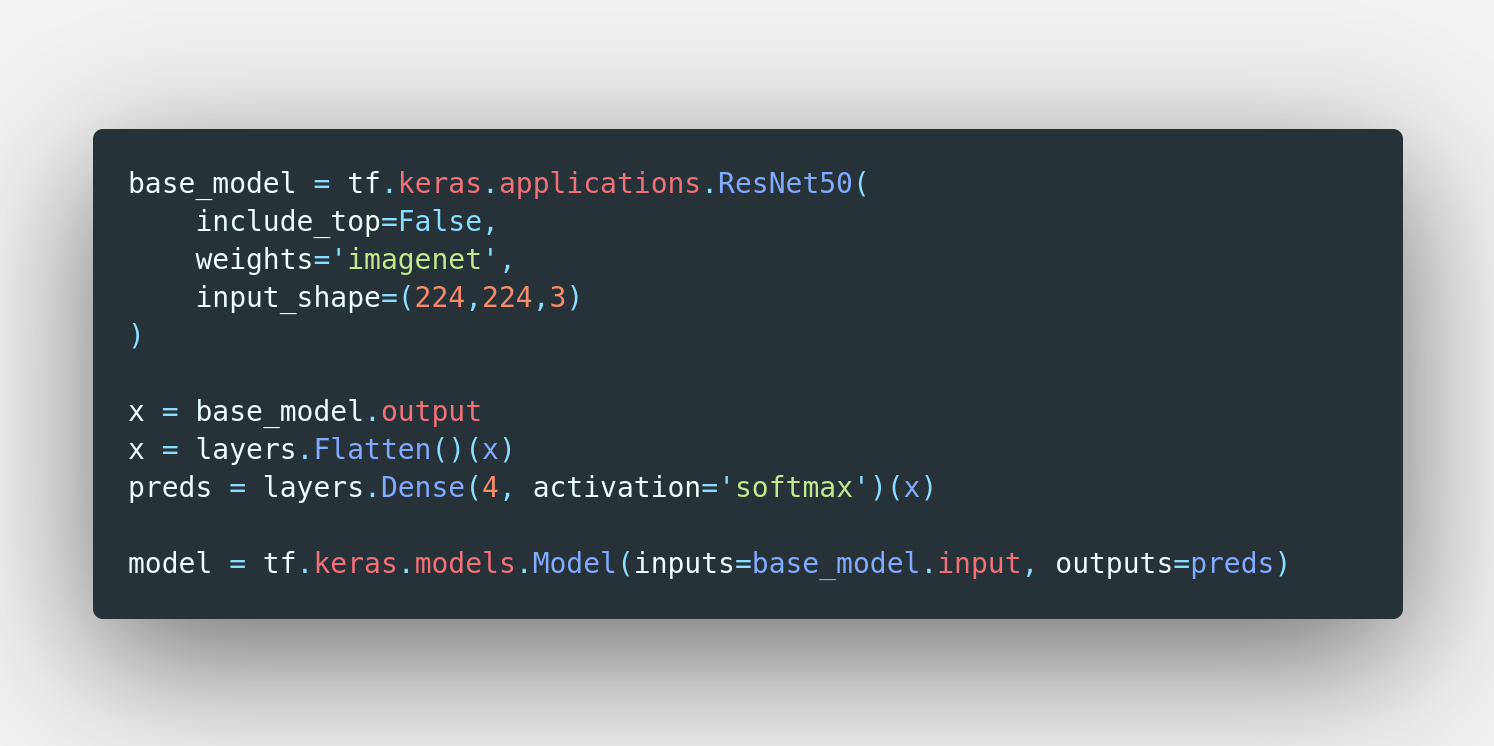
\includegraphics[width=0.8\textwidth]{images/Code/transfer}
	\caption{Transfer Learning Model}
	\label{fig:images-Code-transfer}
\end{figure}

Freezing was used in order to ensure that only the top ``res5c'' block, and the
added classifier block were trainable. This can be seen implemented in Figure
\ref{fig:freeze}.

\begin{figure}[H]
	\centering
	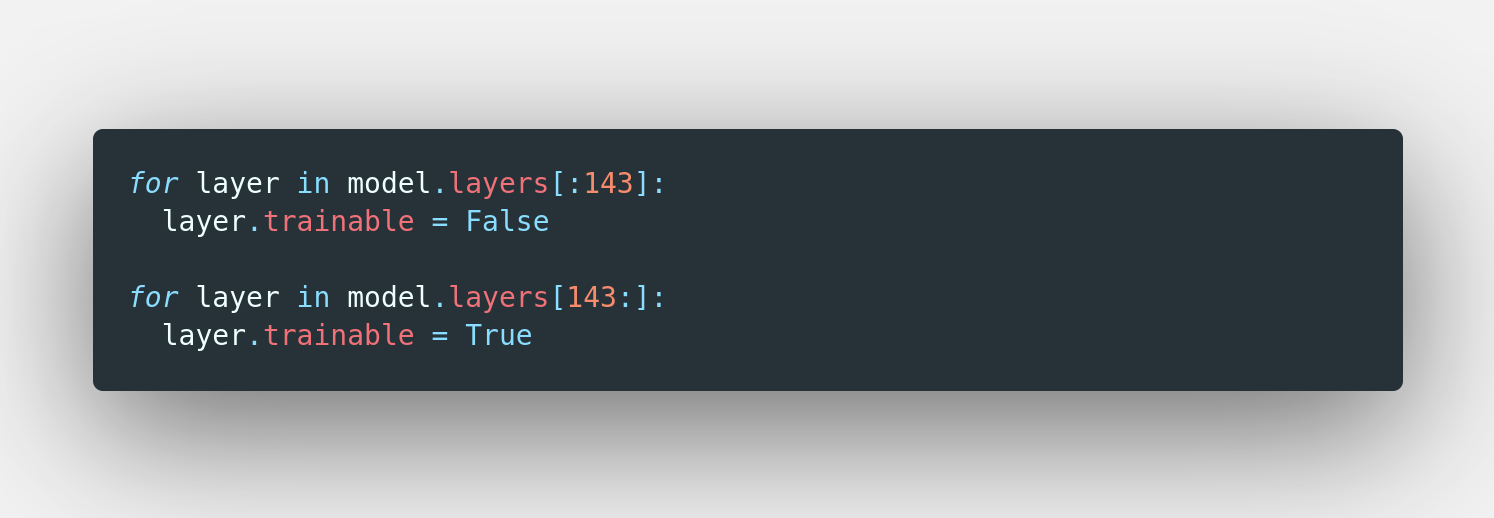
\includegraphics[width=0.8\textwidth]{images/Code/freeze}
	\caption{Freezing the Lower ResNet Layers}
	\label{fig:freeze}
\end{figure}

\subsubsection{Testing}

Testing of the transfer learning portion of this assignment involved only the
addition of the ``Flatten'' and ``Dense'' layers, and as such, no comparisons
between hyperparameters have been made.

\subsubsection{Results}

The final number of layers of the model can be seen in Figure \ref{fig:q2model}.
The added layers, i.e. the ``Flatten'' and ``Dense'' layers are the final output
layers, with the Dense layer classifying the images into one of four classes.

\begin{figure}[H]
	\centering
	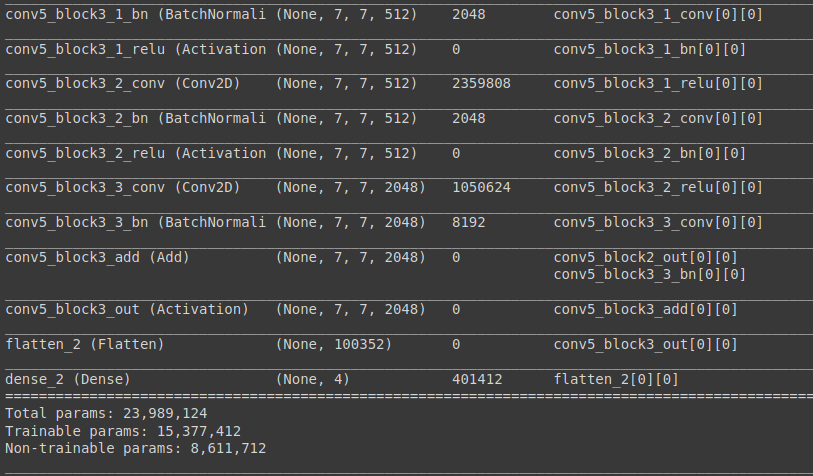
\includegraphics[width=0.8\textwidth]{images/q2/model}
	\caption{Model Summary (Final Layers)}
	\label{fig:q2model}
\end{figure}

There is an obvious difference between the training accuracy and the validation
accuracy, as shown in Figure \ref{fig:q2acc}, and it is clear from this graph
and from the final test results that the model is not overfitting.

\begin{figure}[H]
	\centering
	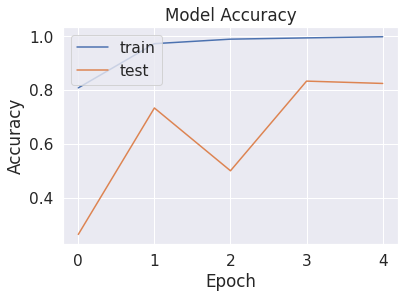
\includegraphics[width=0.8\textwidth]{images/q2/accuracy}
	\caption{Validation and Training Accuracy}
	\label{fig:q2acc}
\end{figure}

The loss for this model, as shown for both the training and validation sets in
Figure \ref{fig:q2loss}, is very low.
Over 5 epochs it can be seen how quickly the value decreases to almost zero.

\begin{figure}[H]
	\centering
	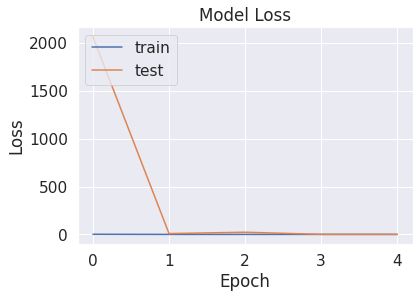
\includegraphics[width=0.8\textwidth]{images/q2/loss}
	\caption{Validation and Training Loss}
	\label{fig:q2loss}
\end{figure}

The final test results from the model can be seen in Figure
\ref{fig:q2results}. The precision has an average value of 83\%, while the
recall has an average value of 86\%. For such a short training time, this value
is much higher than that of Question 1. The highest precision value is for the
``Waffles'' class, however, the recall for this class is the lowest. The highest
recall value is for the ``Omlette'' class, but this has the lowest
precision value. The highest overall value by f1-score is for the ``Hamburger''
class, with a precision value of 91\%, and a recall value of 89\%.

\begin{figure}[H]
	\centering
	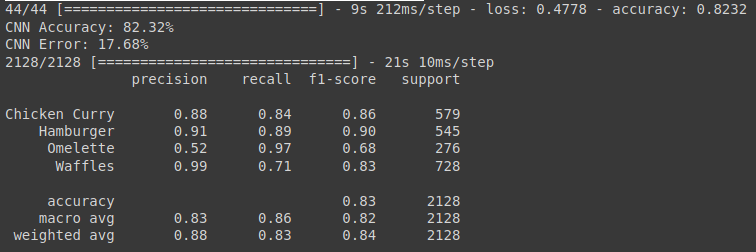
\includegraphics[width=0.8\textwidth]{images/q2/results}
	\caption{Model Testing Results}
	\label{fig:q2results}
\end{figure}

The confusion matrix shows the ``Waffles'' class, labeled as ``3'', as having
the
greatest number of correctly identified samples, while the ``Hamburger'' and
``Chicken Curry'' classes,
labelled ``1'' and ``0'' respectively, as having the least number of
incorrectly identified samples.

\begin{figure}[H]
	\centering
	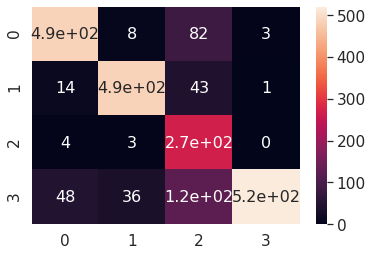
\includegraphics[width=0.8\textwidth]{images/q2/matrix}
	\caption{Confusion Matrix}
	\label{fig:q2matrix}
\end{figure}

The overall training time of this model was 154.2878 seconds. This would give a
value of 0.643lbs of CO2 equivalent emissions. This is much lower than the
developed baseline model in Question 1, and with a much higher output accuracy.

\subsection{Part b}
Part b was left incomplete due to time constraints and a lack of previously
unseen images.

\subsection{Part c}
\subsubsection{Introduction}

The aim of this section is to demonstrate the effects of data augmentation on
the performance of the neural network.

\subsubsection{Rational}

Data augmentation is a technique typically used in order to increase the size of
small datasets. Having more images, with unique features allows for the training
of a more robust neural network. By rotating, mirroring, and scaling images the
neural network can become more robust in real use cases to these variances in
input image.

\subsubsection{Design}

For this section, the values in the ``testDataGenerator'' were modified. The
width shift range and height shift range were given values of 0.1, while the
horizontal and vertical flip arguements were given ``True'' values. The width
shift range and height shift range take a float value and shift the image the
input fraction of the width/height, in this case 1/10th. The horizontal and
vertical flip randomly mirror the image along the horizontal or vertical planes.

\subsubsection{Testing}

As there were no hyperparameters being tested, there was no testing which took
place. The code was executed to extract final data, discussed in the Results
section.

\subsubsection{Results}

The output for the neural network structure is the same as that of Part a, as no
change is being made to the CNN structure, only to the input test data.

\begin{figure}[H]
	\centering
	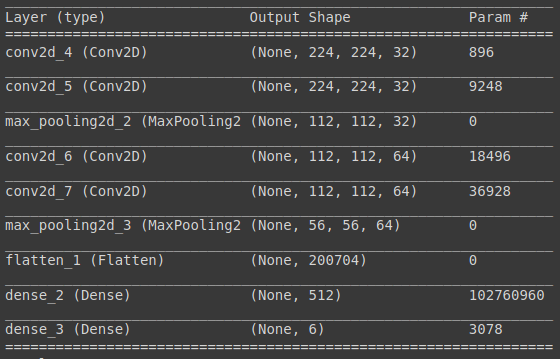
\includegraphics[width=0.8\textwidth]{images/q1/pc/q1pcmodel}
	\caption{Model Summary}
	\label{fig:q1pcmodel}
\end{figure}

Figures \ref{fig:q1pcacc} and \ref{fig:q1pcloss} show that overfitting is not
occurring. While the validation accuracy is quite close to the testing accuracy,
the best fit line through the points on the graph would be below that of the
training accuracy.

\begin{figure}[H]
	\centering
	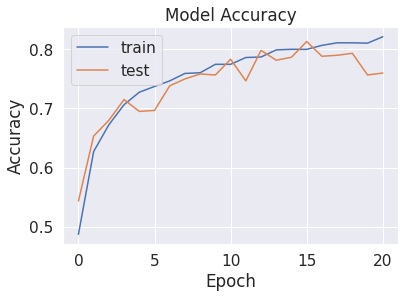
\includegraphics[width=0.8\textwidth]{images/q1/pc/accuracy}
	\caption{Validation and Training Accuracy}
	\label{fig:q1pcacc}
\end{figure}

The loss value improves yet again, with a value of approximately 0.8 in the
validation set.

\begin{figure}[H]
	\centering
	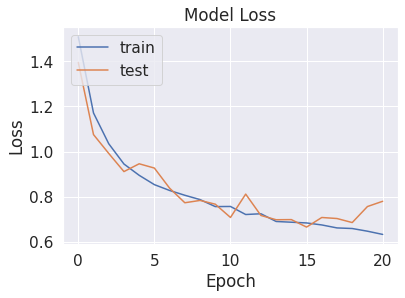
\includegraphics[width=0.8\textwidth]{images/q1/pc/loss}
	\caption{Validation and Training Loss}
	\label{fig:q1pcloss}
\end{figure}

The final output shows an average precision and recall of 85\% and 86\%
respectively , with the highest
values attributed to the ``Parachute'' class, and the lowest values associated
with the ``English Springer'' class.

\begin{figure}[H]
	\centering
	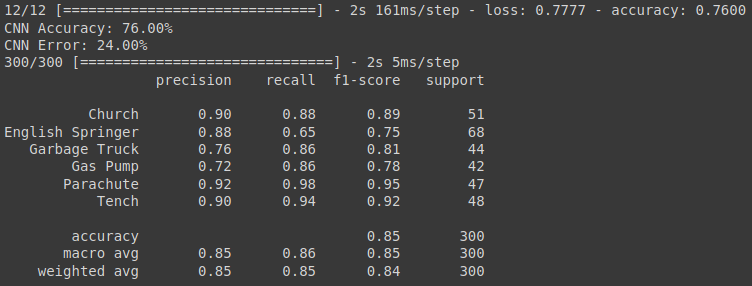
\includegraphics[width=0.8\textwidth]{images/q1/pc/results}
	\caption{Model Testing Results}
	\label{fig:q1pcRes}
\end{figure}

The confusion matrix again demonstrates the number of correctly identified
samples, with the highest precision class being ``Parachute'', labelled as
``4'' within the matrix.

\begin{figure}[H]
	\centering
	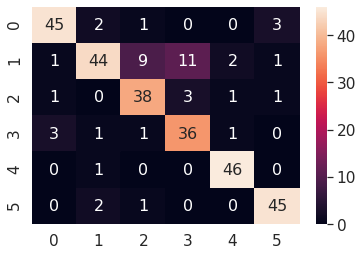
\includegraphics[width=0.8\textwidth]{images/q1/pc/matrix}
	\caption{Confusion Matrix}
	\label{fig:q1pcMatrix}
\end{figure}

Using early stopping, the model ran for a total of 21 epochs. The training time
for this model was 2185.3824 seconds, giving an emission output of 9.106lbs CO2
equivalent emissions. This is, yet again, much higher than Part a, and is also
higher than Part b.

\subsection{Part d}
\subsubsection{Introduction}

This section aims to add batch normalization to the neural network designed in
Part A. The effect on the neural network should be investigated in order to
determine if it increases the performance of the network.

\subsubsection{Rational}

Batch normalization works to alleviate the effects of covariate shift within a
CNN. Batch normalization allows for the use of higher training rates, and also
the use of less dropout within the network, due to the regularization effects it
has.

\subsubsection{Design}

Batch normalization was originally proposed as a layer to be placed before the
activation function, however, it has been noted that performance increases can
be found by placing the layer after the activation function. As the base model
is defined with the activation functions within the layer definitions, the
normalization layers will be placed after the activation functions.

\begin{figure}[H]
	\centering
	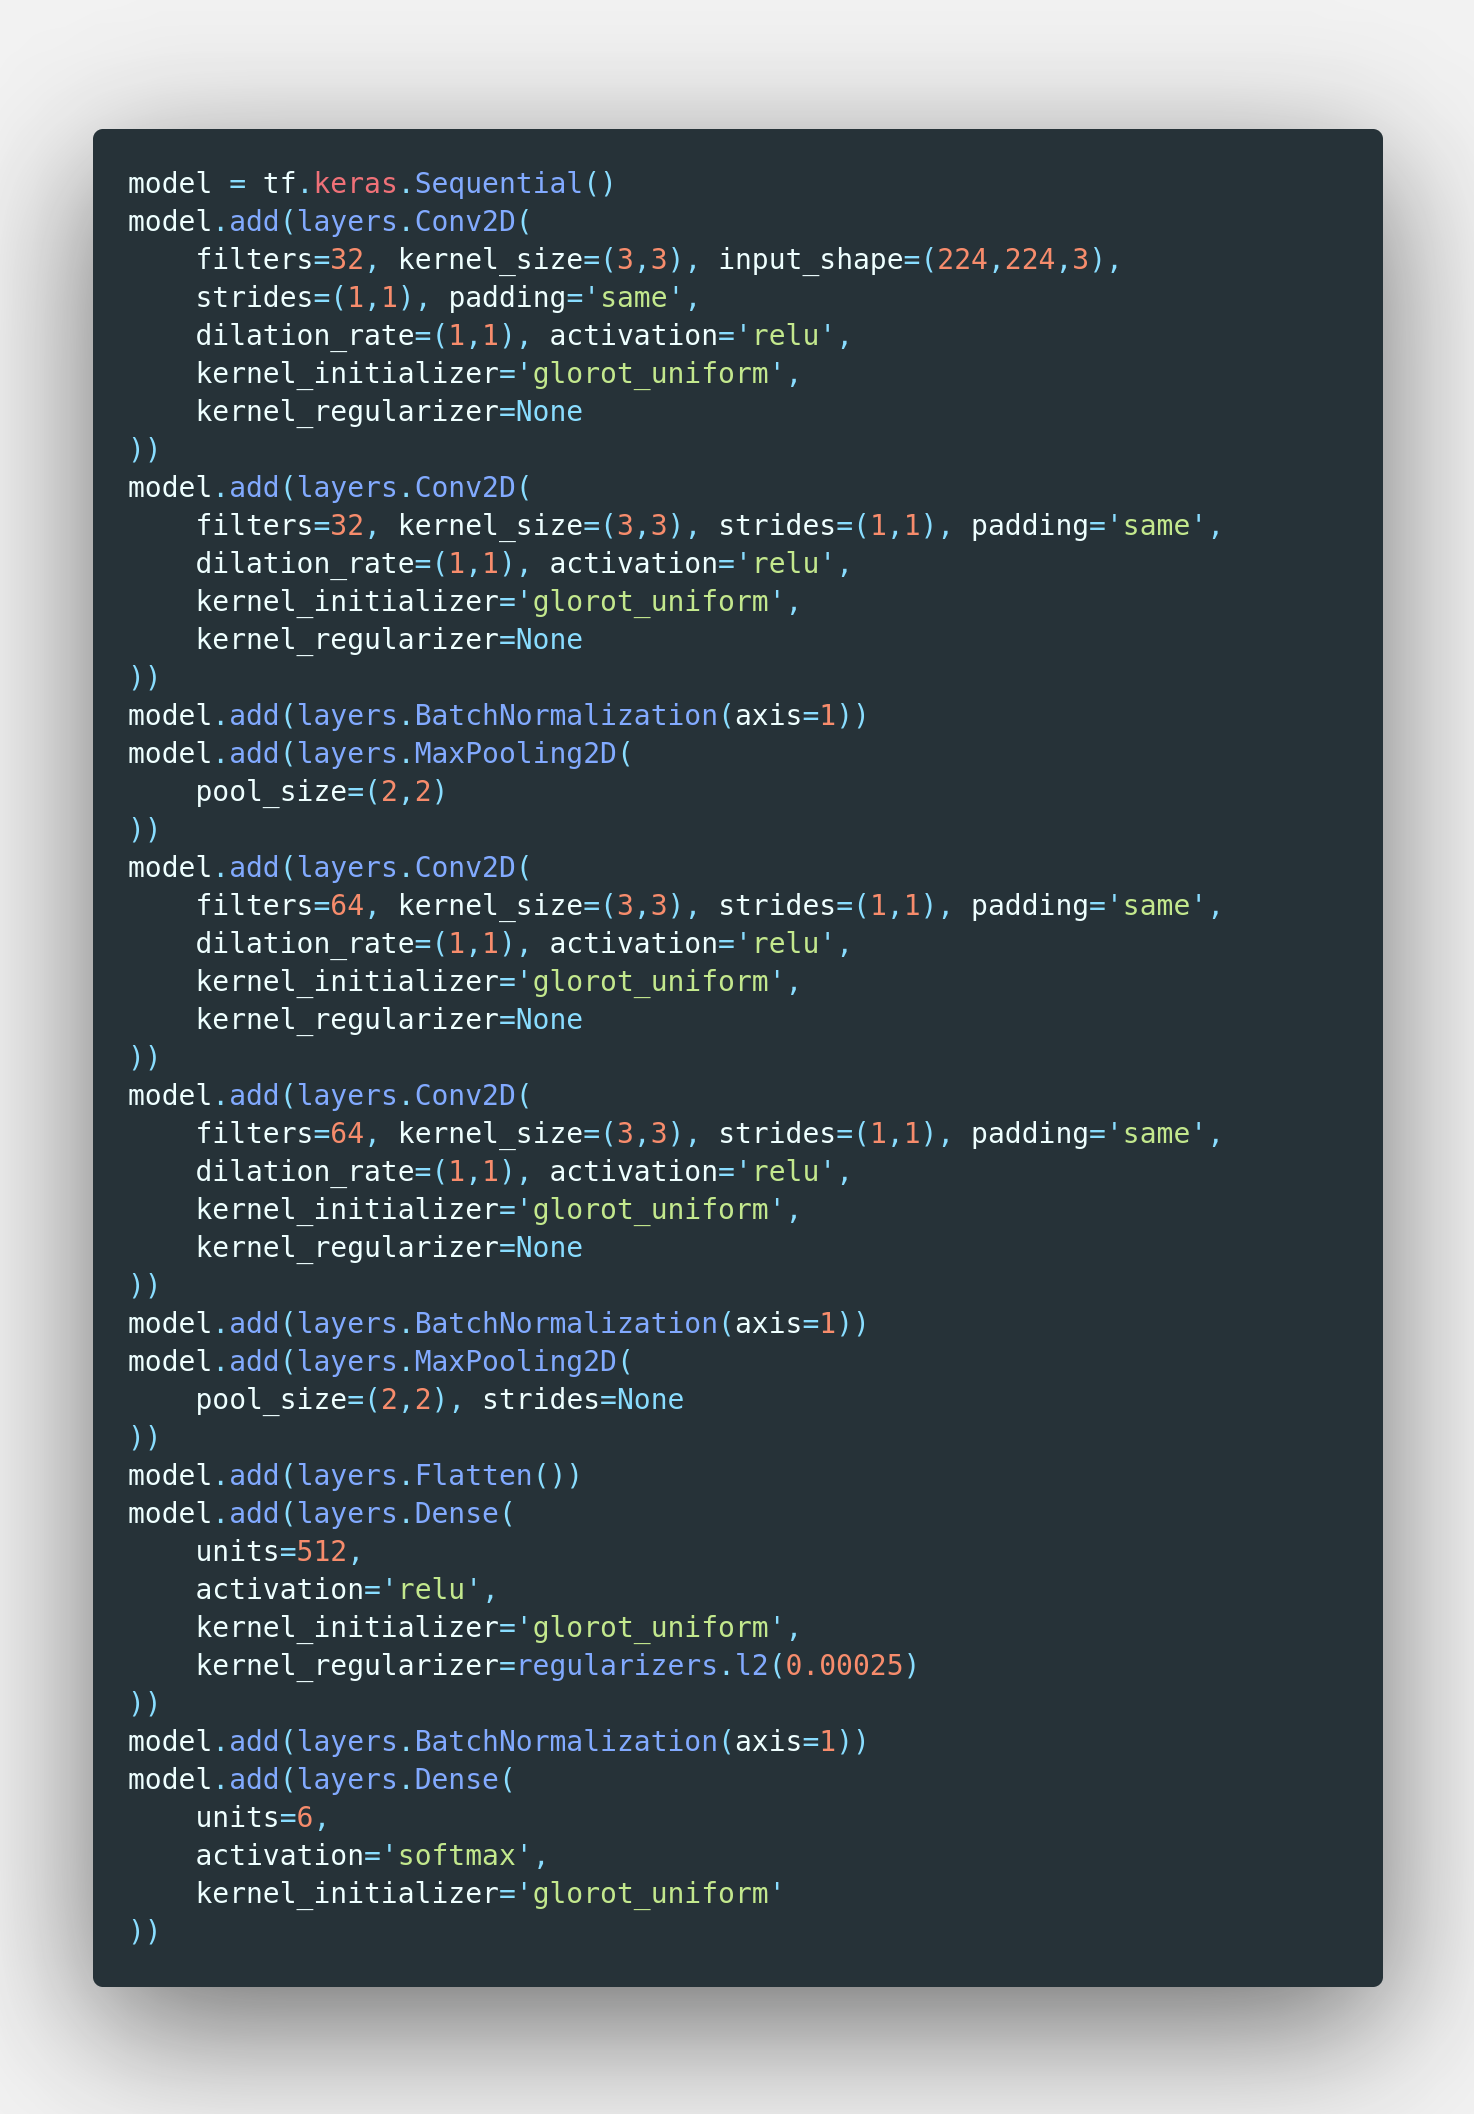
\includegraphics[width=0.8\textwidth]{images/Code/batchnorm}
	\caption{Batch Normalization Model}
	\label{fig:images-Code-batchnorm}
\end{figure}

\subsubsection{Testing}

As previously mentioned, three batch normalization layers were added to the
model. The hyperparameter being tested is the momentum, which, by default is set
to 0.99. The value of 0.5 and 0.0 were also tested, as outlined below.

\begin{table}[H]
	\centering
	\caption{Batch Normalisation Hyperparameter Tuning}
	\label{tab:bnhyp}
	\begin{tabular}{|c|c|}
	\hline
	Momentum & Validation Accuracy \\
	\hline
	0.99 & 78.83 \\
	0.5  & 78.50 \\
	0.0  & 74.33 \\
	\hline
	\end{tabular}
\end{table}

The value of 0.0 for momentum was proposed in the original paper in which batch
normalisation was introduced, however, the default value of 0.99 is shown to
have the best accuracy. As such this is the value which will be tested.

Again, the number of epochs was increased to 30, however, the early stopping
patience value left at 5, as any higher and the model would train for all 30
epochs, and give low accuracy.

\subsubsection{Results}

The model structure, as output via the ``model.summary'' function in keras, can
be seen below. The three batch normalisation layers can clearly be seen.

\begin{figure}[H]
	\centering
	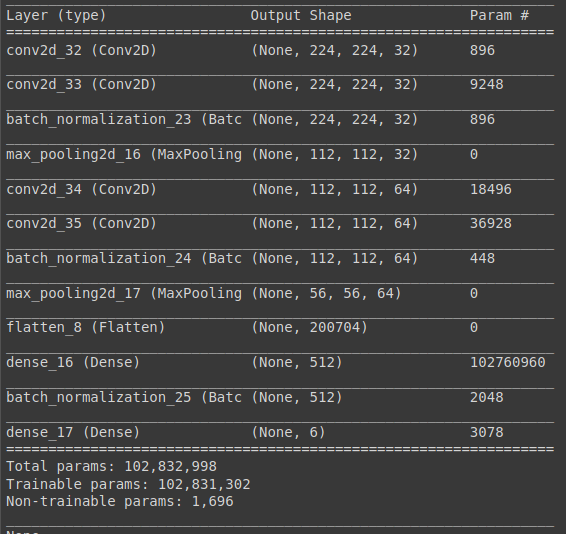
\includegraphics[width=0.8\textwidth]{images/q1/pd/q1pdmodel}
	\caption{Model Summary}
	\label{fig:q1pdmodel}
\end{figure}

The plots in Figures \ref{fig:q1pdacc} and \ref{fig:q1pdloss} show the
validation and training accuracies and losses respectively. The
validation accuracy shows that the model is not overfitting, and the loss is
relatively low.

\begin{figure}[H]
	\centering
	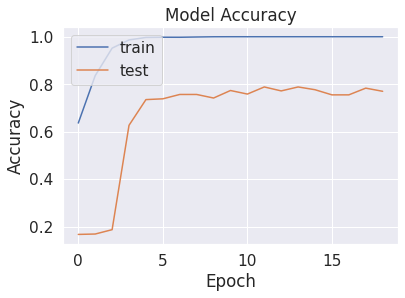
\includegraphics[width=0.8\textwidth]{images/q1/pd/accuracy}
	\caption{Validation and Training Accuracy}
	\label{fig:q1pdacc}
\end{figure}

\begin{figure}[H]
	\centering
	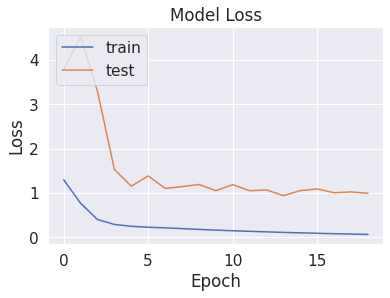
\includegraphics[width=0.8\textwidth]{images/q1/pd/loss}
	\caption{Validation and Training Loss}
	\label{fig:q1pdloss}
\end{figure}

The test output gives an average precision and recall of 80\%, with the highest
values attributed to the ``Parachute'' class, and the lowest values attributed
to the ``English Springer'' class.

\begin{figure}[H]
	\centering
	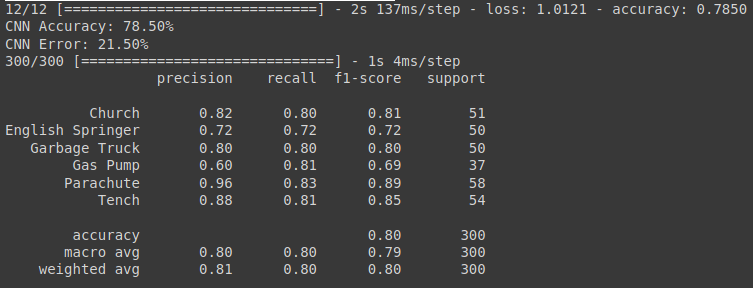
\includegraphics[width=0.8\textwidth]{images/q1/pd/q1pdresults}
	\caption{Model Testing Results}
	\label{fig:q1pdResults}
\end{figure}

The confusion matrix shows the number of correctly identified test samples, with
the highest precision class being ``Parachute'', labelled as ``4'' within the
matrix.

\begin{figure}[H]
	\centering
	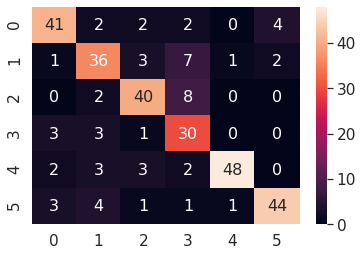
\includegraphics[width=0.8\textwidth]{images/q1/pd/matrix}
	\caption{Confusion Matrix}
	\label{fig:q1pdMatrix}
\end{figure}

Using early stopping, the model ran for a total of 19 epochs, The training time
for this model was 536.67 seconds, giving an emission output of 2.236lbs CO2
equivalent emissions. While this value is lower than Part c, it is higher than
that of Part a and Part b, showing the overhead involved with batch
normalisation.

\subsection{Part e}
\subsubsection{Introduction}

Part e aims to combine the previous sections, applying a combination of dropout,
data augmentation and batch normalization to the baseline model from Part a.
The aim is to develop a CNN with the optimal accuracy.

\subsubsection{Rational}

By combining the advantages of the techniques used in the previous sections,
a CNN can be developed which outperforms the baseline model developed in Part a.
While it is not necessary to utilise all of the techniques, combinations of data
augmentation, dropout, and batch normalisation can lead to improved accuracy
for the neural network.

\subsubsection{Design}

The design of this section came about from the combination of the techniques in
each of the previous sections. As discussed in the Testing section below,
different combinations of the techniques were tested in order to obtain the best
possible accuracy from the model. The final code for this section can be seen in
the appendices.

\begin{figure}[H]
	\centering
	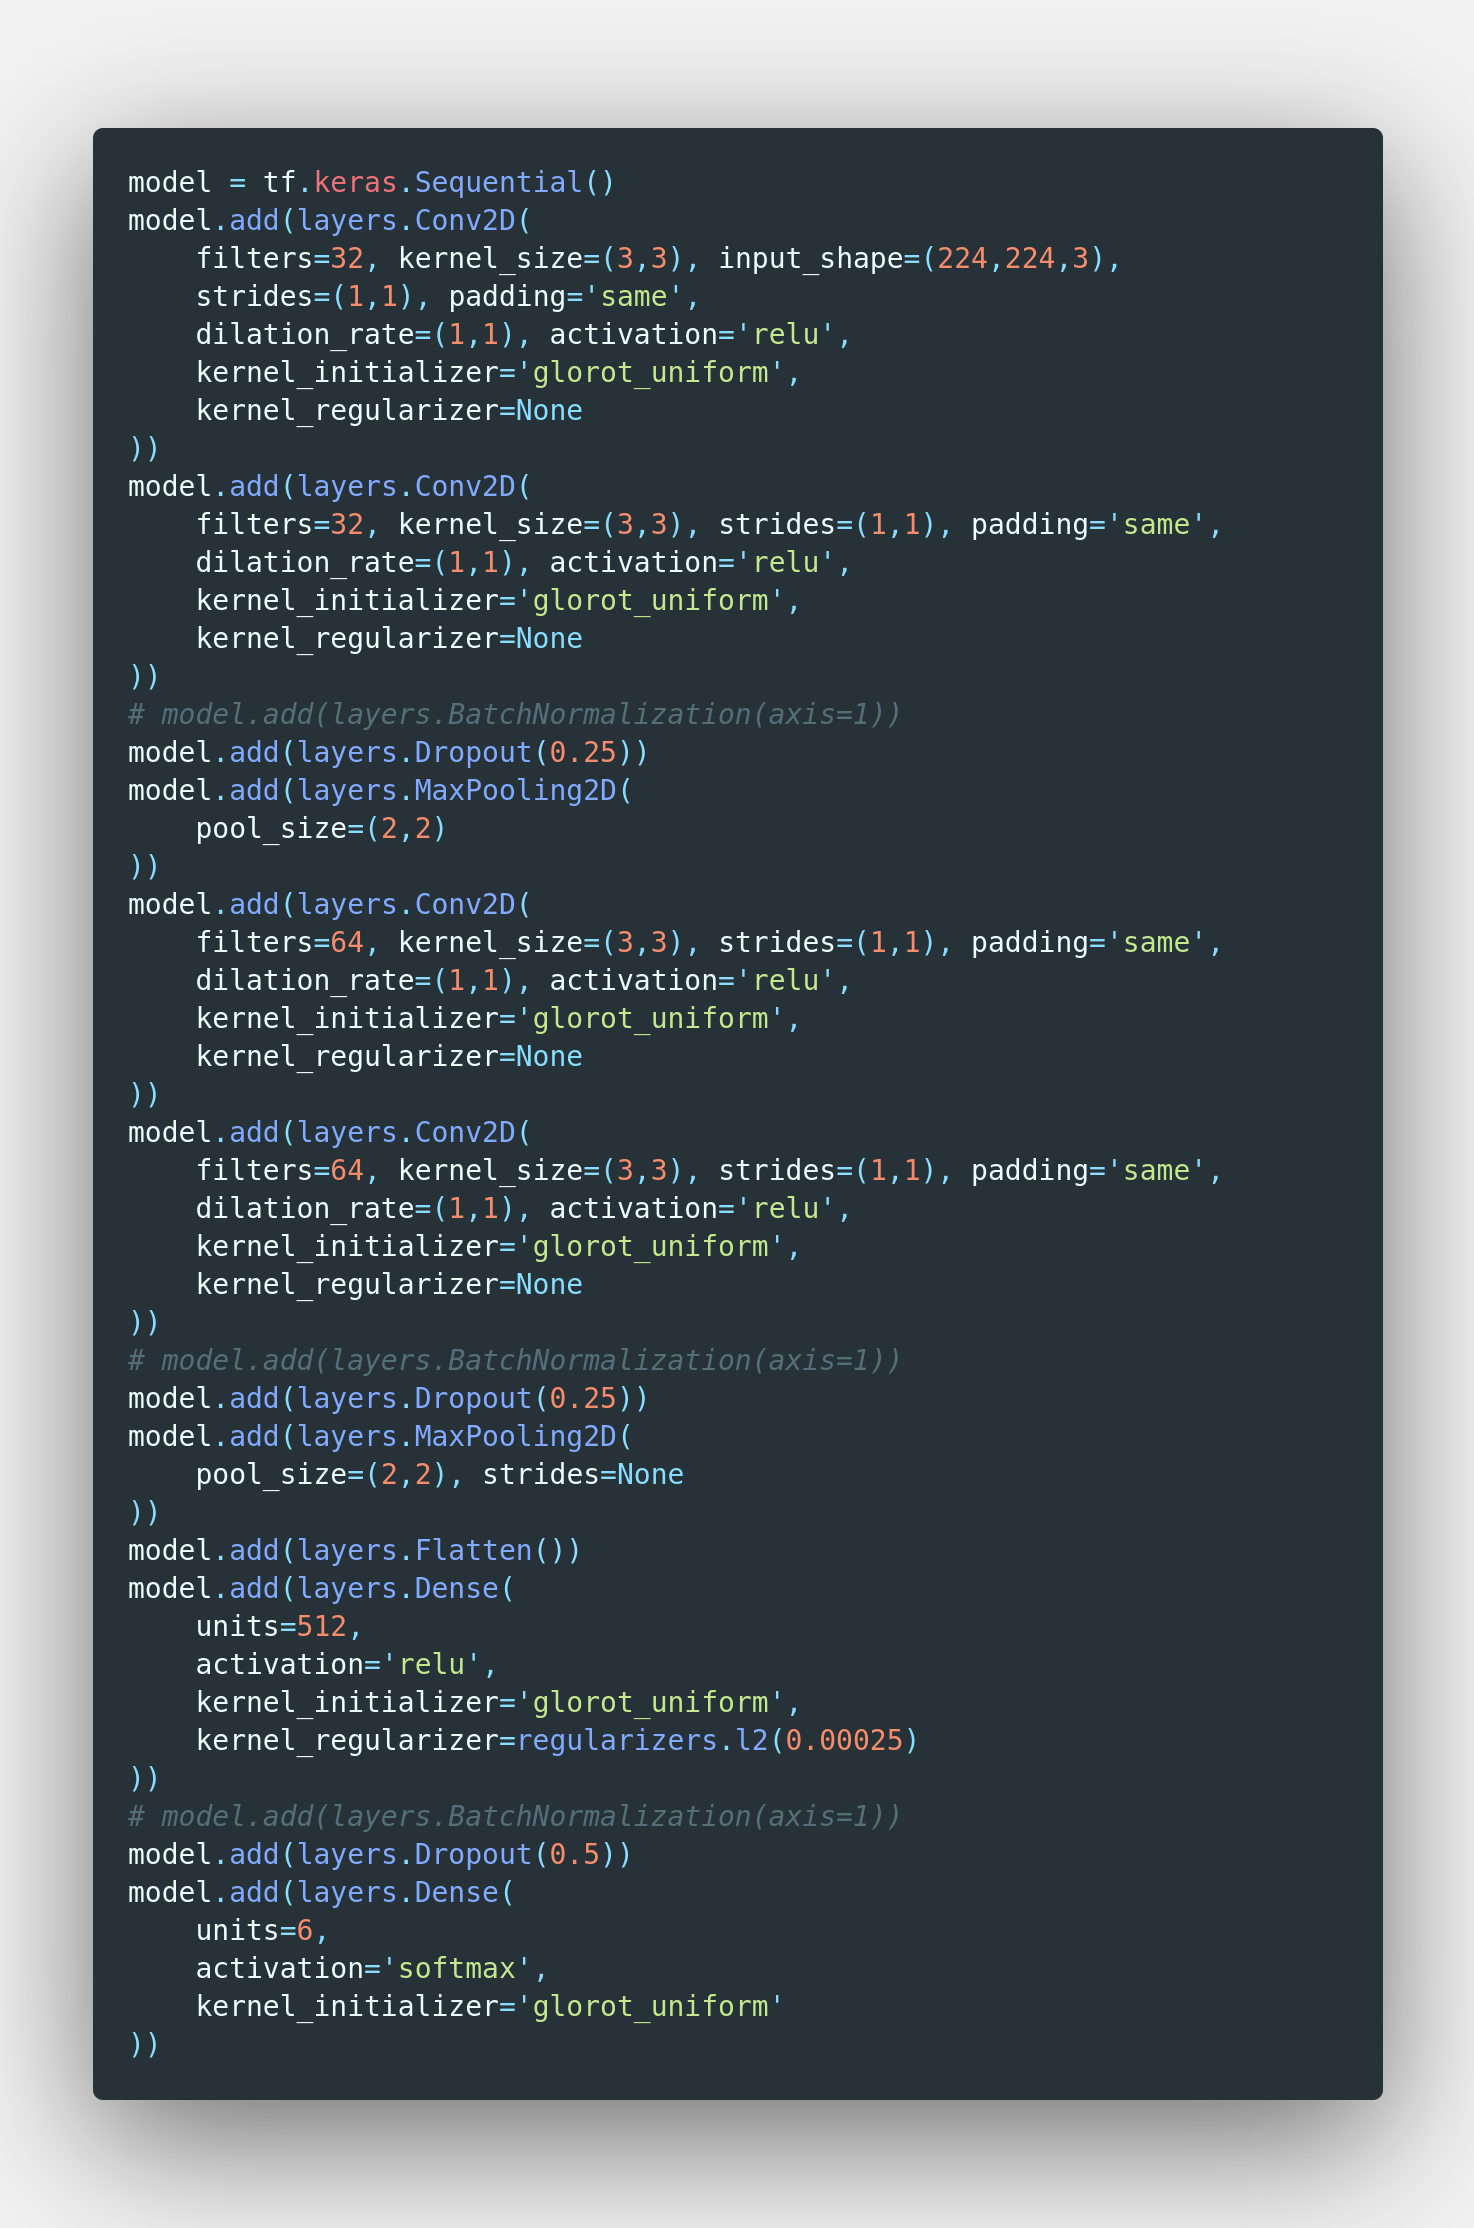
\includegraphics[width=0.8\textwidth]{images/Code/combo}
	\caption{Combined Technique Model}
	\label{fig:images-Code-combo}
\end{figure}

\subsubsection{Testing}

Testing was again done manually, and as such, the obtained result is suboptimal.

\begin{table}[H]
	\centering
	\caption{Layer and HyperParameter Testing}
	\label{tab:q1pe}
	\begin{tabular}{|c|c|}
	\hline
	CNN Description & Validation Accuracy \\
	\hline
	Combined Part a-d & 76.17 \\
	Batch Normalisation + Data Augmentation & 76.17 \\
	Dropout + Data Augmentation & 71.17 \\
	Batch Normalisation + Dropout & 70.5 \\
	No Batch Normalisation in the output layers & 72.5 \\
	No Dropout in the output layers & 66.2 \\
	\hline
	\end{tabular}
\end{table}

By using only Dropout and Data Augmentation , and a dropout rate of 0.25 for
the non-output
Dropout layers, a highest validation accuracy of 78.17\% was achieved. This is
far from optimal, however it is approximately on par with the results obtained
from using Dropout and Data Augmentation separately. This is undoubtably due to
poor hyperparameter tuning.

\subsubsection{Results}

The model summary shown below displays the use of dropout within the model. As
mentioned, data augmentation was also applied to the input images in order to
achieve the performance that is seen in the results.

\begin{figure}[H]
	\centering
	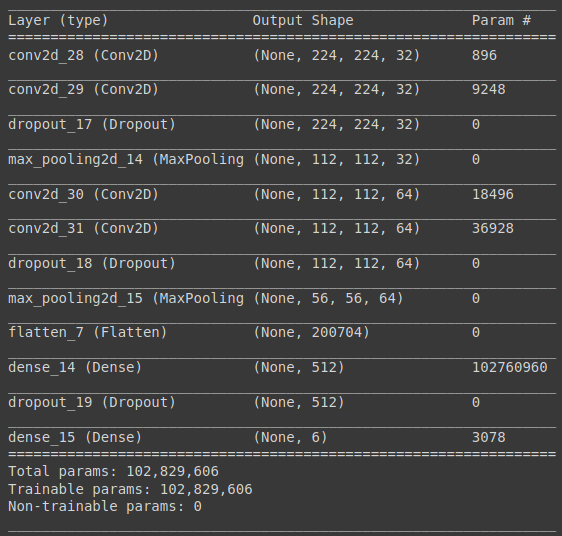
\includegraphics[width=0.8\textwidth]{images/q1/pe/q1pemodel}
	\caption{Model Summary}
	\label{fig:q1pemodel}
\end{figure}

The model seems to be overfitting to the training set. This is an issue as the
training set does not have extremely high accuracy, and this is likely causing
issues with the predictions of the test set.

While the loss is relatively low, the overall accuracy does not benefit from
this improvement in the system.

\begin{figure}[H]
	\centering
	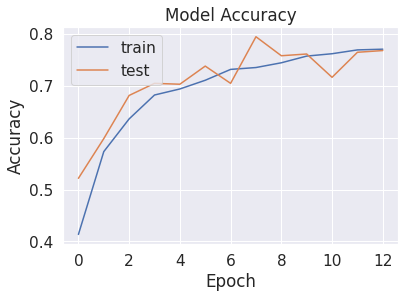
\includegraphics[width=0.8\textwidth]{images/q1/pe/accuracy}
	\caption{Validation and Training Accuracy}
	\label{fig:q1peacc}
\end{figure}


\begin{figure}[H]
	\centering
	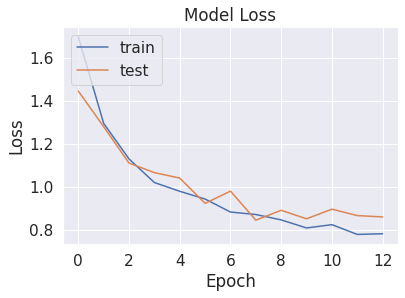
\includegraphics[width=0.8\textwidth]{images/q1/pe/loss}
	\caption{Validation and Training Loss}
	\label{fig:q1peloss}
\end{figure}

The test results can be seen in Figure \ref{fig:q1peresults}. The average
precision is 82\%, while the average recall is 82\%. These values are below the
values achieved using only Data Augmentation techniques. Again, this is likely
due to the poor implementation of hyperparameter tuning, i.e. trial-and-error.

\begin{figure}[H]
	\centering
	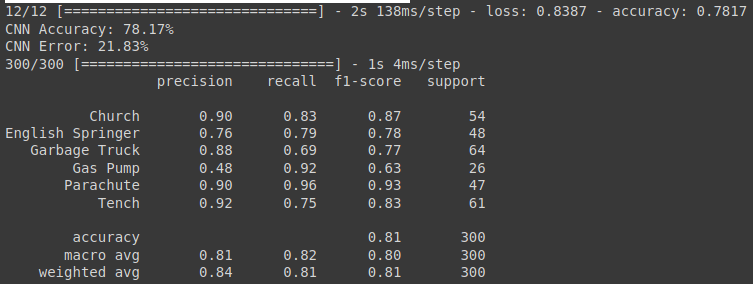
\includegraphics[width=0.8\textwidth]{images/q1/pe/results}
	\caption{Model Testing Results}
	\label{fig:q1peresults}
\end{figure}

The confusion matrix in Figure \ref{fig:q1pematrix} shows that the highest
number of correctly identified samples belonged to the ``Church'' class.

\begin{figure}[H]
	\centering
	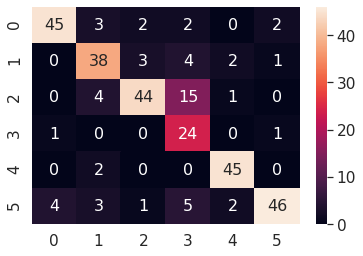
\includegraphics[width=0.8\textwidth]{images/q1/pe/matrix}
	\caption{Confusion Matrix}
	\label{fig:q1pematrix}
\end{figure}

The training time of this model was 1138.7972 seconds, which is 4.745lbs of CO2
equivalent emissions.

\section{Question 2}
The aim of section 2 of this assignment is to implement ``Transfer Learning''
using a Resnet-50 model. The model must be adapted to the ``Food-101''
classification task, classifying images of foods which fall into the following
classes; Chicken Curry, Hamburger, Omelette, and Waffles. The dataset is yet
again pre-divided into training, validation, and test sets, therefore requiring
no pre-processing in order to be divided.

The Keras ``ResNet50'' model is used for this section of the assignment. This
model has 174 layers, as is specified in the assignment brief.

\subsection{Part a}
\subsubsection{Introduction}

The aim of part A is to implement the optimisation of the classification task
using the pretrained ResNet50 model. Fine-tuning based transfer learning is to
be utilised in order to apply the pretrained model to the required task, i.e.
classifying the Food-101 dataset.

\subsubsection{Rational}

Utilising a pretrained model can be useful as a fast way of deploying a neural
network. When using a small dataset, getting high test accuracy can be difficult
to achieve. Transfer learning can be utilised in order to improve the achieved
accuracy. By training only the output layers of the model on the new dataset,
the model can be trained to classify the new dataset to a high degree of
accuracy.

Another benefit of transfer learning is the training time. As the model is
pretrained, and only certain layers are required to be retrained on the new
dataset, the model can be trained in much fewer epochs, meaning that it will
train much quicker than an untrained or newly developed model.

\subsubsection{Design}

The Food-101 dataset is loaded from Google drive in the same way as Question 1.
Once loaded, the ``ImageDataGenerator'' for the training data must have the
``resnet50.preprocess\_input'' function applied. No preprocessing is to be done
to the validation or the test images. The ``flow\_from\_directory'' function is
again used to pull the images from google drive.

The base model for this problem is the keras ``ResNet50'' model. This model
takes the input arguments ``include\_top'', ``weights'', and ``input\_shape''.
Include top defines whether the classifier section of the model is included. As
this problem calls for transfer learning to be applied, this value is set to
False. The weights argument defines what data the model is trained on. Again,
the problem specifies that the ResNet50 model is trained on the ``imagenet''
weights. Finally, the input shape is the dimensions of the input data, which in
this case is 224x224x3.

\begin{figure}[H]
	\centering
	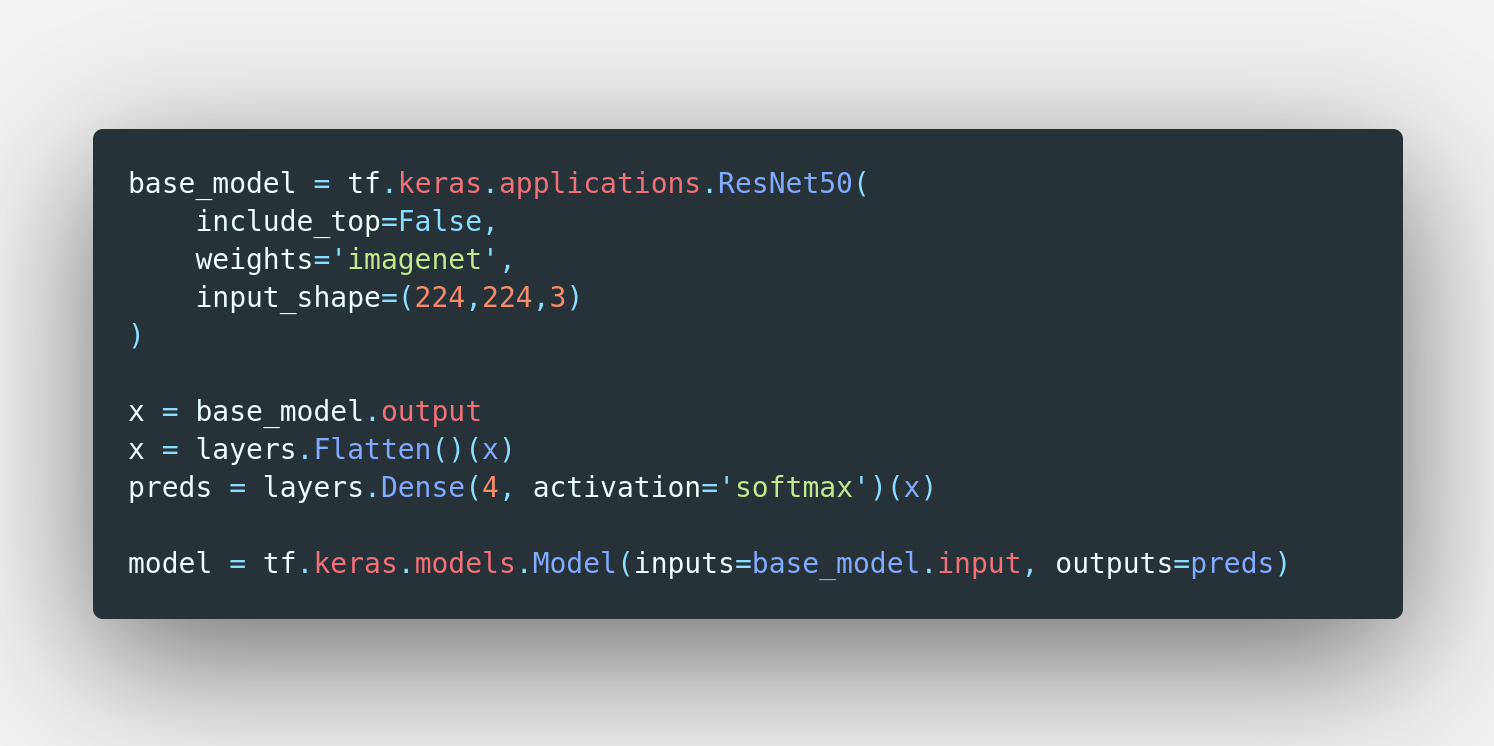
\includegraphics[width=0.8\textwidth]{images/Code/transfer}
	\caption{Transfer Learning Model}
	\label{fig:images-Code-transfer}
\end{figure}

Freezing was used in order to ensure that only the top ``res5c'' block, and the
added classifier block were trainable. This can be seen implemented in Figure
\ref{fig:freeze}.

\begin{figure}[H]
	\centering
	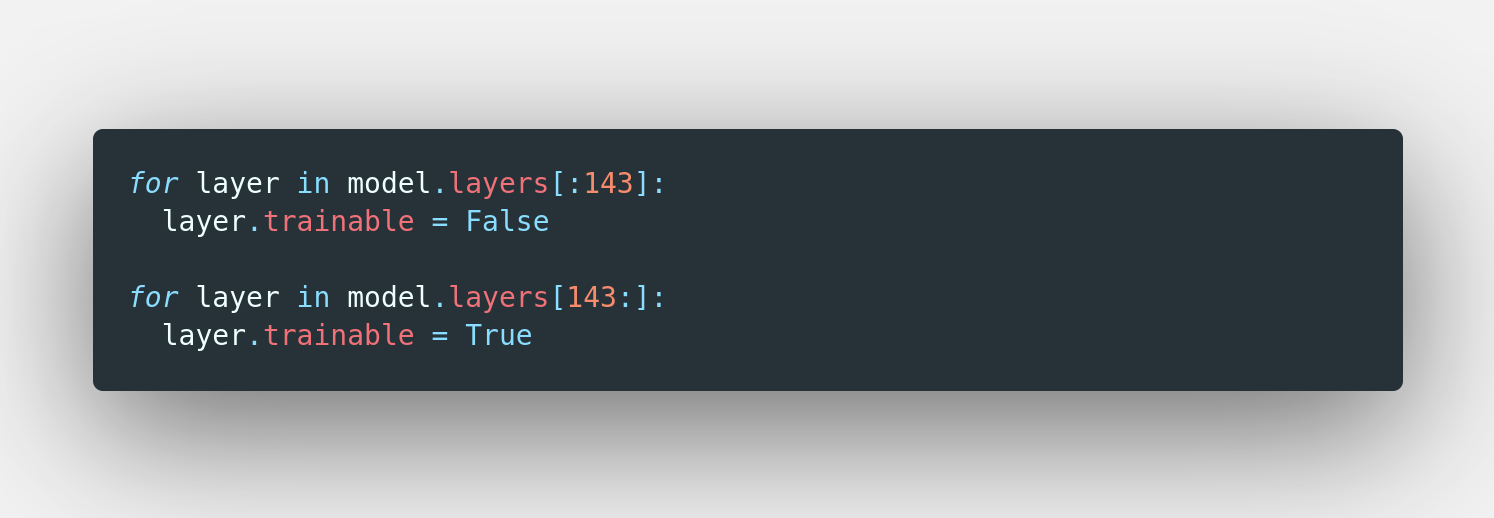
\includegraphics[width=0.8\textwidth]{images/Code/freeze}
	\caption{Freezing the Lower ResNet Layers}
	\label{fig:freeze}
\end{figure}

\subsubsection{Testing}

Testing of the transfer learning portion of this assignment involved only the
addition of the ``Flatten'' and ``Dense'' layers, and as such, no comparisons
between hyperparameters have been made.

\subsubsection{Results}

The final number of layers of the model can be seen in Figure \ref{fig:q2model}.
The added layers, i.e. the ``Flatten'' and ``Dense'' layers are the final output
layers, with the Dense layer classifying the images into one of four classes.

\begin{figure}[H]
	\centering
	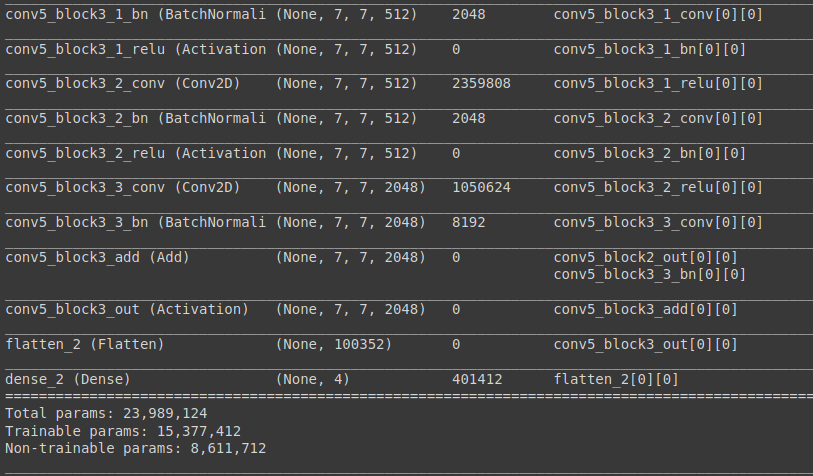
\includegraphics[width=0.8\textwidth]{images/q2/model}
	\caption{Model Summary (Final Layers)}
	\label{fig:q2model}
\end{figure}

There is an obvious difference between the training accuracy and the validation
accuracy, as shown in Figure \ref{fig:q2acc}, and it is clear from this graph
and from the final test results that the model is not overfitting.

\begin{figure}[H]
	\centering
	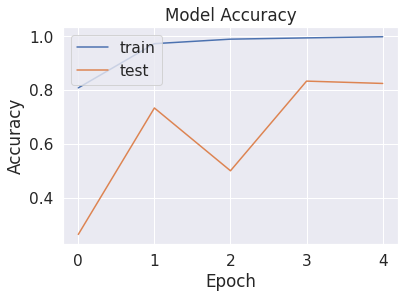
\includegraphics[width=0.8\textwidth]{images/q2/accuracy}
	\caption{Validation and Training Accuracy}
	\label{fig:q2acc}
\end{figure}

The loss for this model, as shown for both the training and validation sets in
Figure \ref{fig:q2loss}, is very low.
Over 5 epochs it can be seen how quickly the value decreases to almost zero.

\begin{figure}[H]
	\centering
	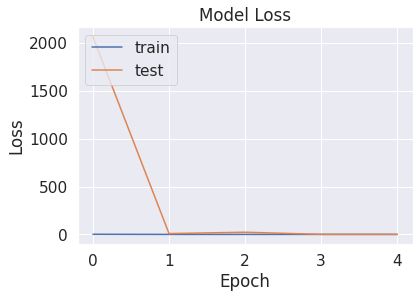
\includegraphics[width=0.8\textwidth]{images/q2/loss}
	\caption{Validation and Training Loss}
	\label{fig:q2loss}
\end{figure}

The final test results from the model can be seen in Figure
\ref{fig:q2results}. The precision has an average value of 83\%, while the
recall has an average value of 86\%. For such a short training time, this value
is much higher than that of Question 1. The highest precision value is for the
``Waffles'' class, however, the recall for this class is the lowest. The highest
recall value is for the ``Omlette'' class, but this has the lowest
precision value. The highest overall value by f1-score is for the ``Hamburger''
class, with a precision value of 91\%, and a recall value of 89\%.

\begin{figure}[H]
	\centering
	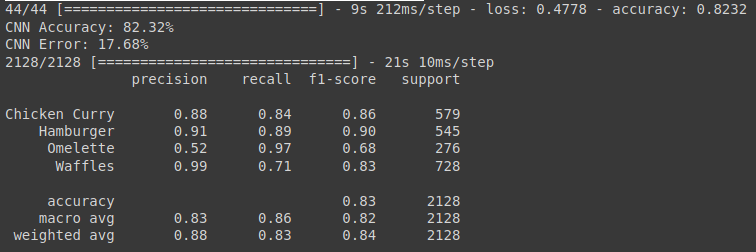
\includegraphics[width=0.8\textwidth]{images/q2/results}
	\caption{Model Testing Results}
	\label{fig:q2results}
\end{figure}

The confusion matrix shows the ``Waffles'' class, labeled as ``3'', as having
the
greatest number of correctly identified samples, while the ``Hamburger'' and
``Chicken Curry'' classes,
labelled ``1'' and ``0'' respectively, as having the least number of
incorrectly identified samples.

\begin{figure}[H]
	\centering
	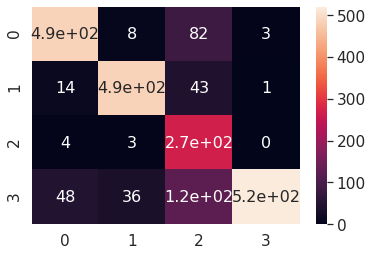
\includegraphics[width=0.8\textwidth]{images/q2/matrix}
	\caption{Confusion Matrix}
	\label{fig:q2matrix}
\end{figure}

The overall training time of this model was 154.2878 seconds. This would give a
value of 0.643lbs of CO2 equivalent emissions. This is much lower than the
developed baseline model in Question 1, and with a much higher output accuracy.

\subsection{Part b}
Part b was left incomplete due to time constraints and a lack of previously
unseen images.

\section{Conclusion}
From the completion of this assignment, it is clear that the task of training a
neural network on a small database is challenging. Attaining high accuracy can
be very difficult. It is also challenging to achieve high accuracy when manually
tuning hyperparameters. A better understanding of automated tools for
hyperperameter tuning, or a better understanding of hyperparameter tuning in
general would undoubtedly have yielded better performance from the model.

Transfer learning proves extremely useful in training a model when given a small
dataset. The ability to take a pretrained model and train a different final
classifier is an excellent way of achieving high accuracy with predictions, as
shown in Question 2 Part a.

The differences in CO2 emissions from training a model with no dropout, data
augmentation, and batch normalisation, to training a model with these techniques
implemented is quite large. However, there is an even more extreme difference to
be seen in using fine-tuning based transfer learning, which had the lowest
emission equivalent value by far. This does not, however, take into account the
training of the model used, but the ability to retrain for different datasets
will cut down on emissions which would otherwise be caused by running hardware
to train newly developed models for every classification task.

\clearpage
\printbibliography
\end{document}
